\chapter{Implementation}
\label{chap:imp}
\lhead{\emph{Project Implementation}}
%This chapter should comprise 15 pages and enumerate your experience when doing what you wanted to do the way you wanted to do it.
The implementation of the system has changed drastically since the original plan due to an oversight where it was believed that the Pistache framework could handle the functionality for both the API and the synchronisation between the tree parity machines. The project turned out to be much more involved and difficult than originally expected. This means that the original sprint plan is no longer representative of the actual sprint plan used. This is however to be expected in an agile environment where the following sprint is normally determined after the evaluation of a sprint that was just completed. Despite all of this the system is functional and produces the same outcome as intended.

\section{Difficulties Encountered}
%Enumerate the different difficulties you have found when developing your solution approach. Create three categories of difficulties:
%\begin{itemize}
%    \item \textbf{Easy}: You managed to solve the problem with little difficulty.
%    \item \textbf{Medium}: It was not easy to solve, but you managed to develop a workaround or solution and %still achieve the functionality you originally had in mind.
%    \item \textbf{Hard}: The difficulty was so complicated that you didn’t managed to solve it. As a result, some functional requirement / non-functional requirement or use case from your solution approach was not achieved.
%\end{itemize}

%For each difficulty, classify it into easy, medium or hard. Then, provide the following info:
%\begin{enumerate}
%    \item Description of the difficulty: Brief description of the problem you found.
%    \item How did it affect the original project design?: Indicate how this difficulty affected:
%    \begin{enumerate}
%        \item the architecture of your solution
%        \item if it represented a risk to your project
%        \item if it affected your methodology to develop your project
%        \item if it changed your implementation schedule
%        \item if it changed the evaluation plan
%    \item What did you do to manage the difficulty arisen?: Brief description of your decision to overcome the %difficulty.
%    \end{enumerate}
%\end{enumerate}
The major difficulties I encountered were primarily related to the architecture of the project. The initial class diagrams were way too basic and didn't account for the fact that Pistache would now only be used for the API and nothing else. 

\textbf{Easy Difficulty}
\begin{enumerate}
\item The NodeJs module was replaced with simply a NodeJs App. The NodeJS module is not implemented due to a time constraint and is not necessary to the outcome of the project. The NodeJs module was originally meant to simplify the communication with the API for people who wish to use it. A NodeJS App would need to be implemented regardless in order to use that module and demonstrate the usability of the API. 
The API doesn't have many routes to use therefore it would not be difficult to use the API with any NodeJs App as interacting with the API is simply done with POST requests. The final NodeJs App that is in the same GitHub repository, consumes the API perfectly as well as purposely demonstrating some aspects of dynamic cryptography that would normally be hidden. Any user that wishes to use the API can simply copy the functions in the NodeJs App that interact with the API and change them accordingly to send and receive their own data. It is recommended for users to copy said functions as there are specific steps that need to take place to register the NodeJS App with the API in particular the synchronisation service. For this reason The NodeJs App uses pure NodeJs libraries like ExpressJs \cite{ExpressJS} which is the most popular routing framework for NodeJs. The NodeJs App has no front end as it would be difficult for users wishing to use the API to adapt the front end too, therefore only a basic HTML template engine is used to deal with the HTML. JavaScript for the front end is purely used for visual purposes and is not required since all of the information sent from the browser to the NodeJs app is done through classic HTML forms. This doesn't have any impact on the architecture as the NodeJS App is not really included in the architecture as it is simply designed to consume the API. This does impact the schedule in a positive way as it is easier and quicker to simply make a NodeJS App than a NodeJs module and a NodeJs App.
\end{enumerate}

\textbf{Medium Difficulty}
\begin{enumerate}
\item The sprints needed to be adjusted to accommodate the new implementation plan. The final sprint plan will be placed here as it briefly reflects the major changes that took place, these changes will be discussed in more detail in the following sections. The Sprint plan follows a two week sprint approach.
\begin{table}[h]
\centering
\caption{New Sprint Plan}
\begin{tabular}{|p{1cm}|p{12cm}|}
\hline Sprint & Tasks \\ [14pt]

\hline 1 & Create a basic API server that can process GET and POST requests. Familiarise self with RapidJSON library \cite{rapidjson} and create functions to parse C++ objects into JSON "strings" and JSON "strings" back into C++ objects. Research peer to peer libraries, no useful ones were found. Decided to make a custom one with the help of the Boost ASIO \cite{boost_asio_home} library. Never used Boost ASIO before therefore a decision was made to follow the developers tutorials on the Boost ASIO website. This was not enough to understand the complicated library therefore other tutorials such as this one \cite{boost_asio_totorial_1} were also followed.  \\ [12pt]

\hline 2 & Further knowledge of Boost ASIO needed to be acquired before it was possible to proceed with coding the actual peer to peer network. Thankfully a very informative book called Boost.Asio C++ Network Programming \cite{boost_book} by John Torjo was purchased and ended up being the last resource needed in order to complete the peer to peer network. A basic peer to peer network was written however was unstable at the end of this sprint \\ [12pt]

\hline 3 & Peer to peer network works as expected. Implemented basic synchronisation with real tree parity machines. Implemented command line parsing using Boost Program Options \cite{boost_asio_cmd} to enable different options such as selective outputs and port configurations. Completed synchronisation between tree parity machines fully therefore they produce the same weights successfully. Implemented "logging" to external terminal windows. \\ [12pt]

\hline 4 & Research how to proceed with the API i.e have two separate processes or contain the API and peer to peer network within the same process. Decision was made to contain both in the same process for security reasons. Basic API server was constructed and could be easily spawned along side the peer to peer service.\\ [12pt]

\hline 5 & Implement API functionality for synchronisation. Changes needed to be made to the peer to peer service to accommodate unexpected requirements needed to begin synchronisation when using the API. AES encryption decryption implemented using Crypto++ \cite{cryptopp} library. Encrypted data needed to be encoded using base64 again with the help of Crypto++ library. Implement a NodeJs app to consume and demonstrate various features of the API.\\ [12pt]

\hline 5 & Test the system. Implement options to choose which parts of the system to log since logging everything at once can be difficult to demonstrate different aspects of the system. Clean up the code. Document instructions on how to setup the system in the GitHub Readme file. \\ [12pt]

\hline
\end{tabular} \\
\label{tab:ProjRisks}
\end{table}

\FloatBarrier


\item The API and the synchronisation could not be done using only the Pistache framework as originally believed. This was a fairly significant set back since I have experimented before with Pistache framework and was familiar with how it operated functionality wise. It was only until I attempted to use Pistache for synchronisation I discovered that my original plan will not work since Pistache is a very good REST framework and not much else. To synchronise the tree parity machines a peer to peer network seemed most appropriate in how the synchronisation was envisioned to take place. After searching for easy to use libraries that supported peer to peer networks nothing that matched the requirements was found. This lead to the conclusion that a custom peer to peer network would have to be built from scratch. The attention grew towards Boost Asio as it is the most flexible generic networking library for C++. Unfortunately this library is quite extensive and is not as abstract as some of the previous peer to peer libraries encountered. Since with Boost Asio you will still deal with sockets however this will allow for greater control provided you know how the library works and Boost Asio has excellent asynchronous support which is essential for a responsive server. It took almost two full sprints to learn how the library works which set my initial schedule back as it was planned to spend time to learn the new technologies that would be used however it was not expected to spend so much time learning said new technologies. However some of the lost time was made back since the design of the peer to peer network was simple and efficient which allowed for a large number of synchronisation requests to take place per second resulting in generating a valid key in around one second which satisfies the requirement and no further optimisations needed to take place. This occurrence changed the architecture significantly since originally this wasn't meant to be present. Overall I'm glad that this happened as I had a chance to learn one of C++'s most popular networking library. Another benefit of using Boost Asio for synchronisation over Pistache apart from the fact that its impossible to achieve using Pistache is because the Boost Asio library is a lot lighter the performance increase is rather large. Obviously this would be impossible to test fairly however based on Pistache stress tests it can manage roughly 300 - 400 requests per second. The peer to peer Boost Asio can process around one thousand requests per second as it takes around one thousand requests for the tree parity machines to synchronise and they synchronise generally once per second.

\end{enumerate}


\textbf{Hard Difficulty}
\begin{enumerate}
\item A major difficulty that has prevented the implementation of a non functional requirement was the ability to use multiple tree parity machines per peer. Originally the plan was to implement multiple tree parity machines per peer, however in practice after spending more than a week on the problem a decision was made to move on and only allow one tree parity machine per peer. This theoretically does not have any impact on performance and certainly has no impact on security. A single tree parity machine per communication works as expected, a peer can have multiple tree parity machines where for example peer1 communicates with peer2 and peer3 at the same time. In this scenario peer1 would have two tree parity machines as the peer will communicate with two other peers. This scenario works flawlessly in the final implementation of the project. If the original plan were to be implemented peer1 would have twenty tree parity machines, ten per peer it communicates to. The reason why this is difficult is because the ten tree parity machines are reading and writing to the same socket. Whereas with one tree parity machine it has exclusive read and write access to the socket. An attempt was made to implement multiple read and write buffers, a queue, custom read and write objects however a decision was made to abandon this feature for now as it took up too much time and didn't add anything beneficial to the project apart from "being cool". 
The architecture of the project can be said to have changed although it is insignificant as the number of tree parity machines is rather virtual in nature. This issue did not represent any major risk to the project as everything works perfectly with one tree parity machine per connection. The implementation schedule was affected as a lot of time was spent on a feature that did not get implemented and it is better to spend time on features that actually do get implemented.
\end{enumerate}



\section{Actual Solution Approach}
In December of last year, when writing the first version of the report, in Chapter 4 you came up with your original solution approach. On it, you presented (i) the architecture of your solution, (ii) your list of use cases, (iii) a risk assessment, (iv) a methodology to develop your solution approach, (v) your implementation schedule, (vi) your evaluation plan and (vii) some prototype of the resulting product. From January to April you have been developing your solution approach. Along the way you have encountered difficulties (the ones listed in Section 5.1) which might have modified your original plan so that you can come up with an actual developed project.

This section is effectively the production of "as built" specification where you compare your original design to the final finished project. Please go section by section (the ones listed from (i) to (vii) in the last paragraph. For each section, enumerate any difference between the original design and the final project, and justify the difficulty forcing you to make such this change. Do not fret if some of these changes are radical, what is important here is that there is a clear rationale for changes made.

\begin{figure}[!h]
  \centering
      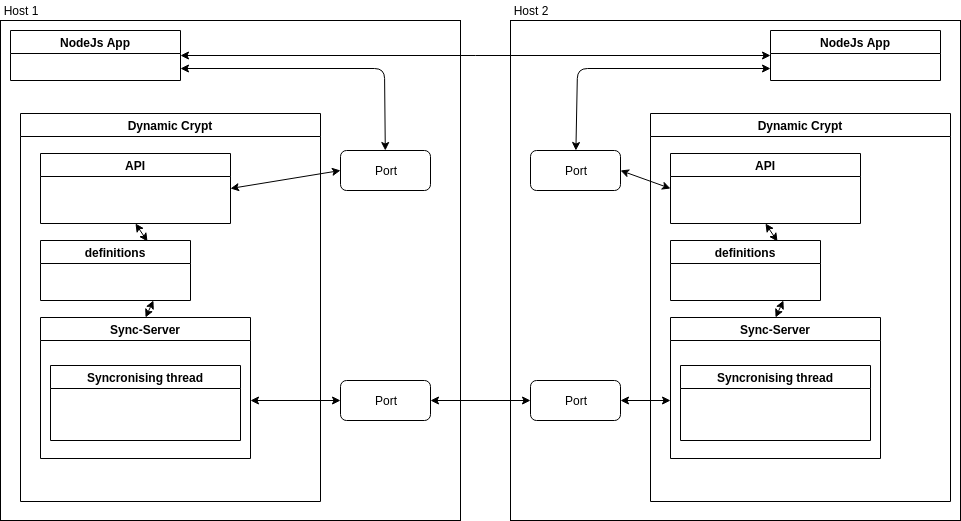
\includegraphics[width=1\textwidth]{Figures/basic-2hosts-final.png}
  \caption[High level overview of architecture]{High level overview of architecture}
  \label{fig:basic-two-hosts-final}
\end{figure}
\FloatBarrier

\begin{figure}[!h]
  \centering
      \includegraphics[width=1\textwidth]{Figures/class-diagram-all-croped.png}
  \caption[DynamiCrypt Class Diagram]{DynamiCrypt Class Diagram}
  \label{fig:class-diagram-all}
\end{figure}
\FloatBarrier

\begin{figure}[!h]
  \centering
      \includegraphics[width=1\textwidth]{Figures/API_class_Diagram-croped.png}
  \caption[DynamiCrypt API Class Diagram]{DynamiCrypt API Class Diagram}
  \label{fig:API_class_Diagram}
\end{figure}
\FloatBarrier

\begin{figure}[!h]
  \centering
      \includegraphics[width=1\textwidth]{Figures/class_diagram_dynamicrypt-part1.png}
  \caption[DynamiCrypt Class Diagram part 1]{DynamiCrypt Class Diagram part 1}
  \label{fig:class_diagram_dynamicrypt-part1}
\end{figure}
\FloatBarrier

\begin{figure}[!h]
  \centering
      \includegraphics[width=1\textwidth]{Figures/class_diagram_dynamicrypt-part2-croped.png}
  \caption[DynamiCrypt Class Diagram part 2]{DynamiCrypt Class Diagram part 2}
  \label{fig:class_diagram_dynamicrypt-part2}
\end{figure}
\FloatBarrier

\begin{figure}[!h]
  \centering
      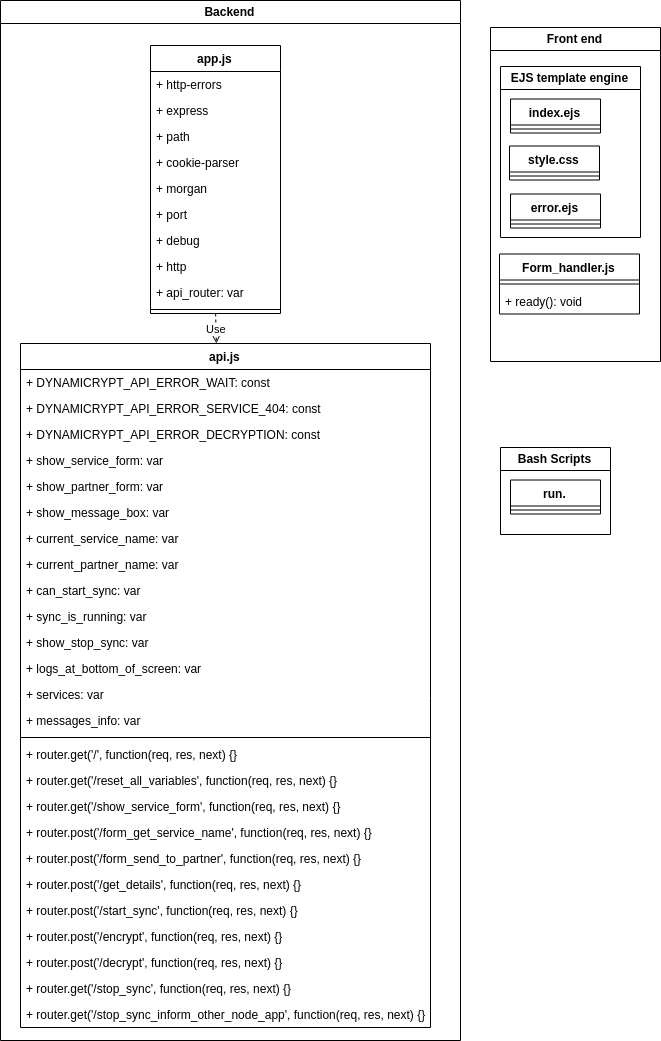
\includegraphics[width=1\textwidth]{Figures/nodeJsApp.png}
  \caption[NodeJs App architecture]{NodeJs App architecture}
  \label{fig:nodeJsApp_architecture}
\end{figure}
\FloatBarrier